\chapter{Introduction}
In computer science, machine learning is a set of methods for learning models from examples that accurately perform tasks on new or unseen data without explicitly codifying all instructions. This automation of programming provides a time- and cost-effective alternative to otherwise manually created software solutions, making machine learning popular and widely used for many applications.

However, the relative lack of human supervision in their creation makes it hard to fully understand the inner workings of trained models and limits the ability to verify that the models work correctly. Even though it is possible to statistically verify the correctness of a model by testing it against an unseen dataset whose ground truth is known, models can unknowingly utilize latent variables that should not be used. Knowledge about those factors is often implicit in the domain of the task and neither encoded in the data nor the model. Human expertise is needed to detect and encode them explicitly or to block them out.

\todo{State core contributions}

\todo{outline of introduction}

%%%
%  Furthermore, a formalization or taxonomy of common machine learning modeling \emph{errors} in both the modeling and feature engineering steps is needed to fully determine the limitations of the proposed black-box analysis methodologies. This can be achieved by taking a survey with both machine learning and domain experts to get an understanding and relevance of different kinds of those errors.
%%%

% Machine learning is a powerful tool that is used more and more in everyday life.
% By relating independent features and targets by detecting complex associations machine learning
% helps human decision making and, in some cases, even replaces it.
% Predictive modeling using classification techniques is a very common application of machine learning.
% In this work we will primarily focus on classification but the techniques discussed can, to some extent, be
% applied in other areas of machine learning as well.

% \begin{figure}
\centering
\vphantom{7cm}
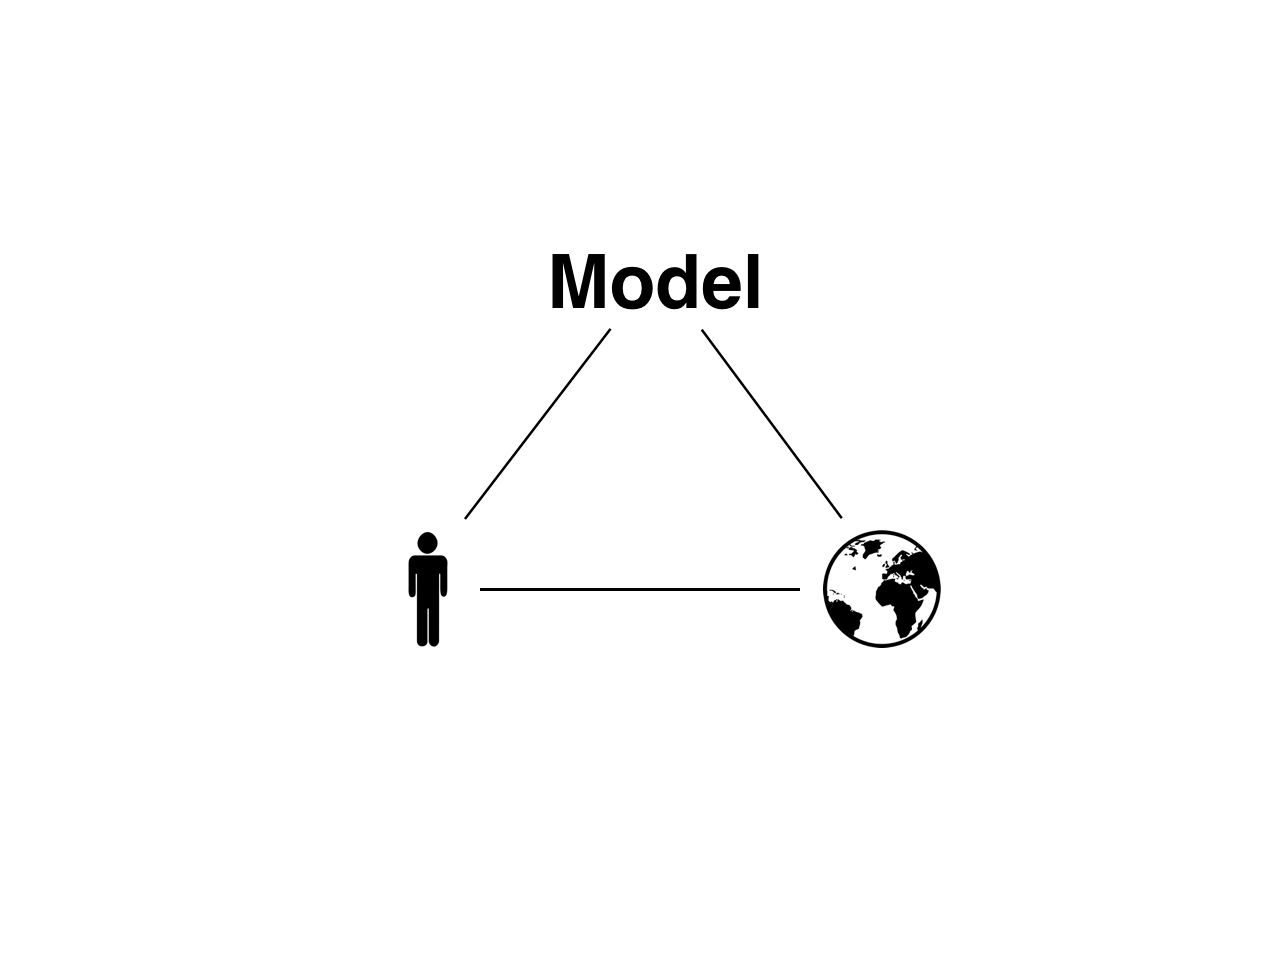
\includegraphics[trim={7cm 8cm 7cm 8cm},clip=true,width=0.275\linewidth]{figs/motivation/hmr}
~
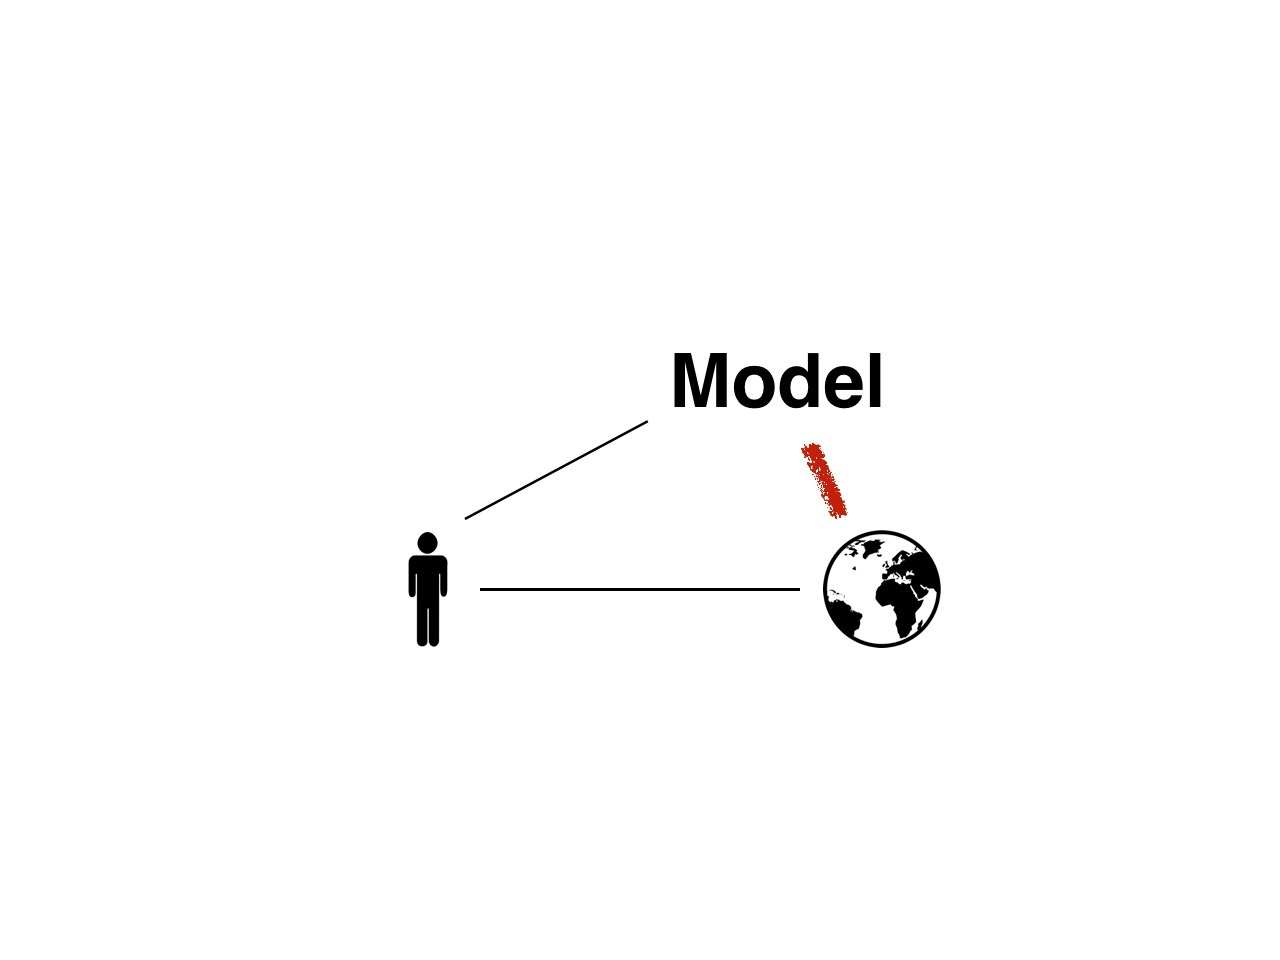
\includegraphics[trim={7cm 8cm 7cm 8cm},clip=true,width=0.275\linewidth]{figs/motivation/hmr_complex}
~
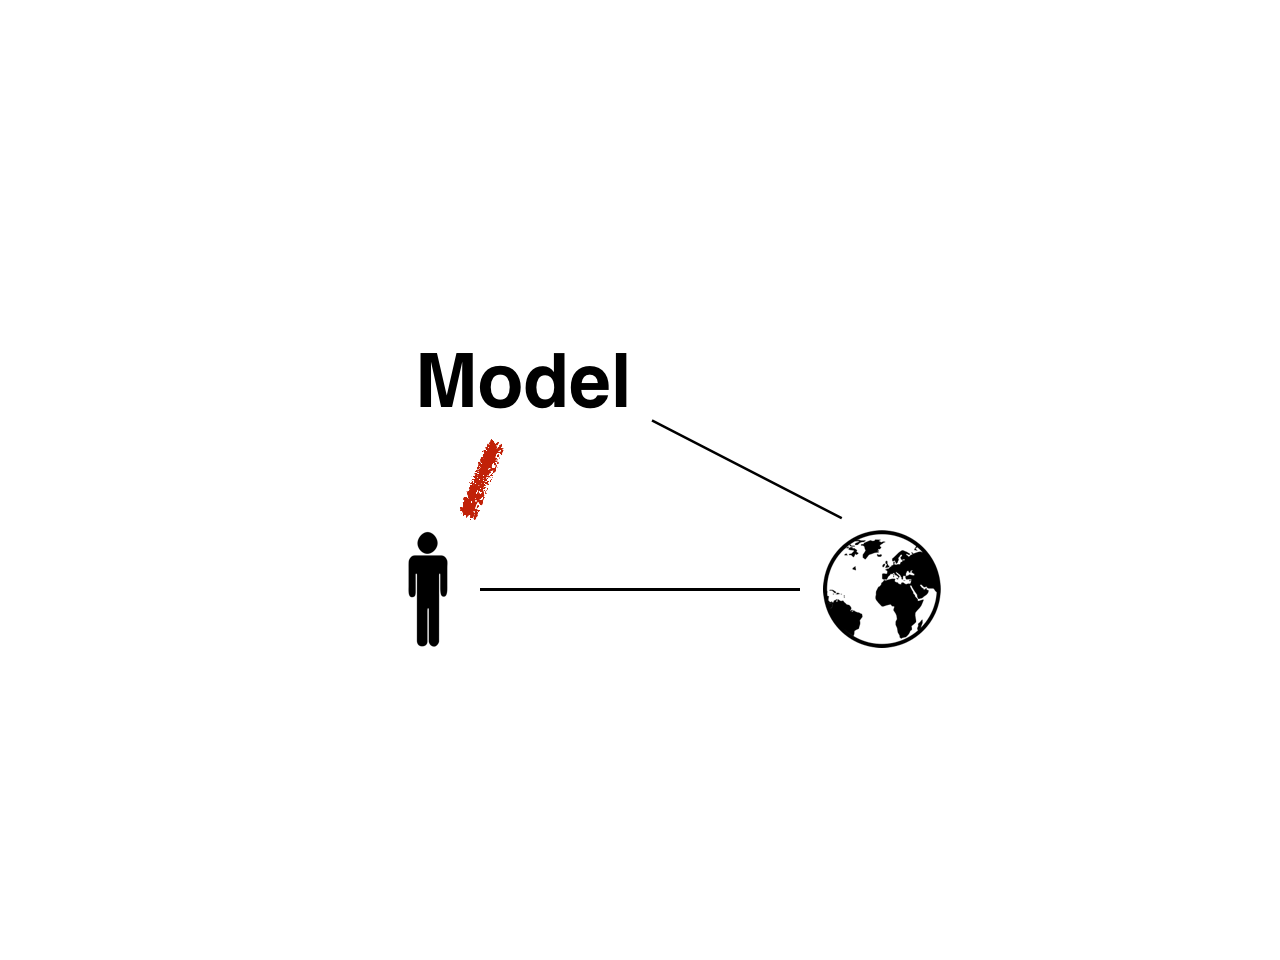
\includegraphics[trim={7cm 8cm 7cm 8cm},clip=true,width=0.275\linewidth]{figs/motivation/hmr_interpretable}
\caption{
Humans (lower left) build machine learning models (top) to understand and
predict reality (lower right). The second image illustrates how improving
machine learning models (ie., closing the gap between the model and reality)
makes it harder for humans to understand it. Likewise, simplifying the model
(ie., closing the gap between the model and the human) makes the model less
accurate (third image).
}
\label{figs:motivation_hmr}
\end{figure}

% As the scope and usage of machine predictions increases with bigger and more complex data
% the used algorithms need to also become more complex.
% However, as complexity increases it becomes harder for humans to follow the machine's decision making
% as illustrated in \figref{figs:motivation_hmr}.
% This problem of model transparency and interpretation is important and very well recognized in machine learning,
% as models with high predictive performance generally have low transparency and vice-versa~\cite{breiman2001}.

% \begin{figure}
\centering

\includegraphics[height=10.5em]{figs/motivation/ml_orig}
\raisebox{4.75em}{$\Rightarrow$}
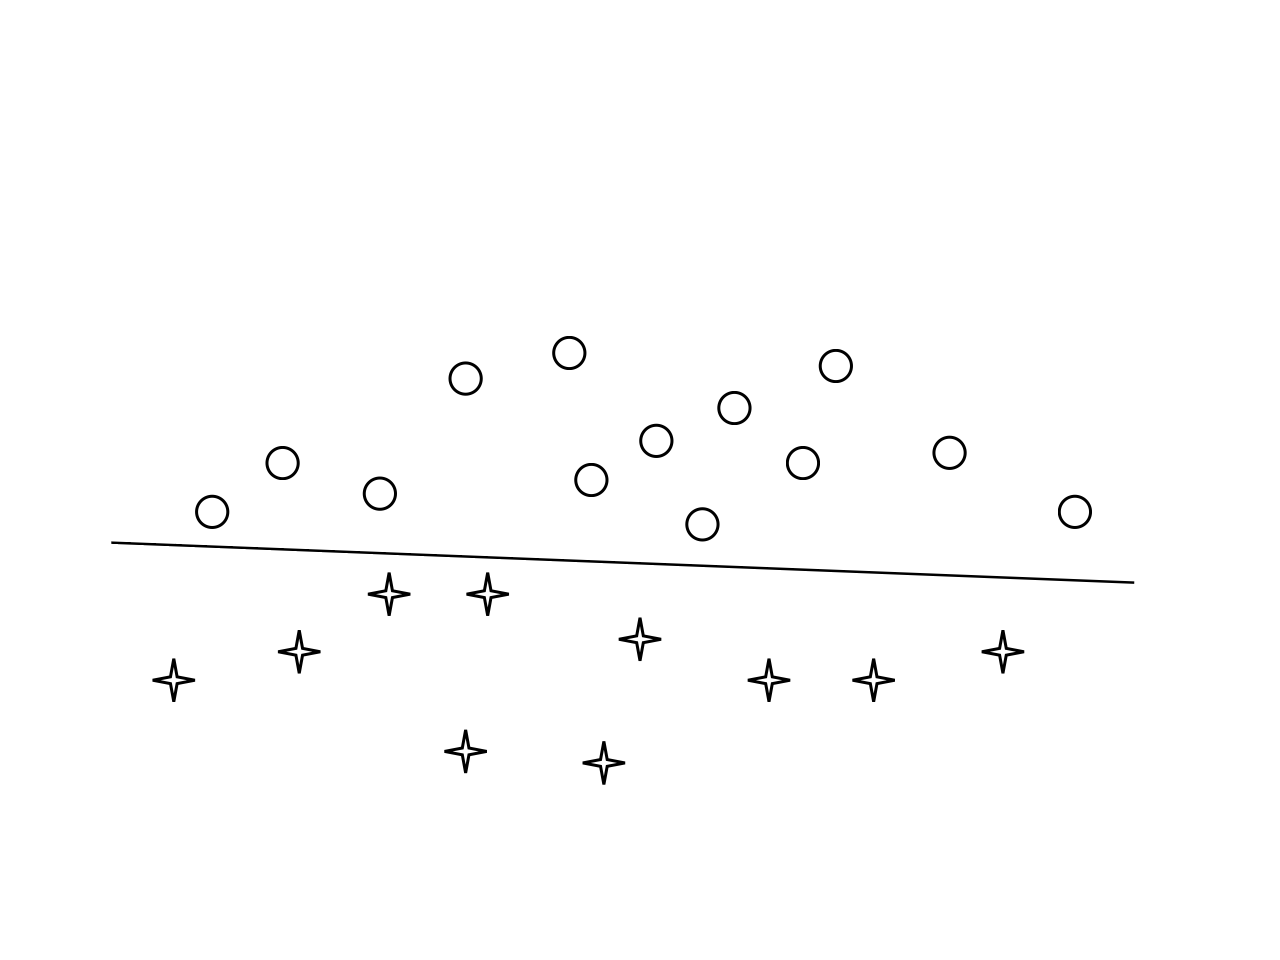
\includegraphics[height=10.5em]{figs/motivation/ml_proj}
\caption{
Machine learning algorithms transform the complex raw input space (left)
into a cleaner transformed space (right) that can be easily separated.
Transformations are often strongly non-linear, non-affine, and/or non-continuous
and thus not easy to follow or understand.
}
\label{figs:motivation_ml}
\end{figure}

% Many applications of machine learning need to be interpretable to humans even though
% sacrificing prediction performance is not desirable.
% For example, in the health care domain disease prediction using patient histories needs to be fully
% transparent and comprehensible to practitioners as lives are at stake when applying models in the real world.
% Even if a model performs well on the test data it could draw its conclusions from hidden signals or biases
% in the training data. We found many of such examples in the work presented here.

% One way of overcoming the problem of interpretability vs. performance in machine learning is to
% break down the complex models into smaller parts that are easier to understand (see \figref{figs:motivation_ml}).
% While this reduces the complexity it also reduces the generalizability of the explanations created this way.
% In the following we will explore when explanations are useful and how they can be used.

% \section{Explanations}
% Explanations for machine learning can be desirable for multiple reasons:

% \begin{description}
%     \item[Liability]
%         Decisions made by the machine have real world consequences with attached liabilities.
%         Explanations are needed to create confidence that the model avoids costly misjudgements of critical inputs.
%     \item[Trust]
%         Stakeholders need to be able to trust decisions from the model.
%     \item[Debugging]
%         Help understanding why a model behaves different than expected.
%     \item[Comparison]
%         Provide a model agnostic way of comparing different models.
%     \item[Hidden Associations]
%         Find hidden associations in the original data.
%     \item[Ambiguity Reduction]
%         By creating generalizing models and explaining their behavior a noise-free view of the data can be created.
% \end{description}

% Those explanation tasks can be performed at different steps in the machine learning process.
% In this context predictive modeling typically consists of three steps (see \figref{figs:motivation_flow}).
% First, the input data has to be prepared.
% This entails choosing which data points are eligible for modeling to ensure that no inherent biases influence
% the validity of the created model.
% Furthermore, data usually needs to be converted into features that can be used by machine learning models.
% Second, the model has to be trained on the transformed data.
% Depending on the type of the model or strategy this step includes splitting the data into cross-validation sets,
% algorithmic feature selection, and actually training the model.
% Third, the actual prediction can be performed which often entails converting class probabilities into
% concrete labels upon which decisions can be performed.

% Explanations can be separated into different categories that utilize and describe
% different stages of the predictive modeling pipeline.
% Thus, explanations can be divided into input-, output-, interaction-,
% and structure-explanations.
% Input explanations mostly work with the raw input data and can help the pre-processing.
% Output explanations analyze outputs from the machine learning model such as feature ranks
% or prediction scores.
% Interaction explanations change model inputs to observe how the corresponding model output
% changes.
% Structure explanations describe the inner values and weights of a model so decisions
% can be followed manually.

% \begin{figure}[b!]
\centering
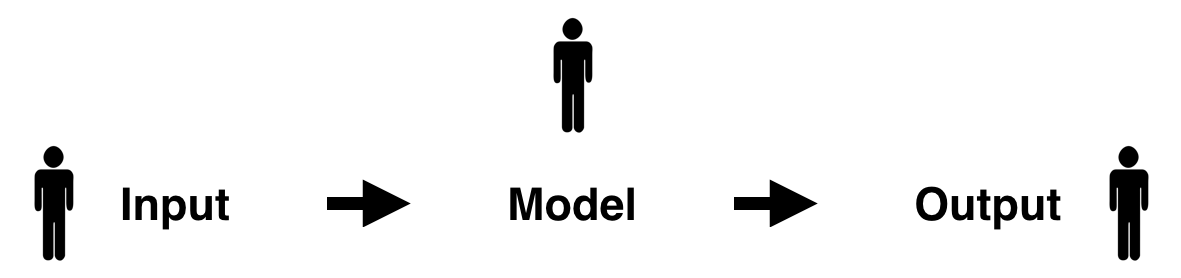
\includegraphics[width=0.7\linewidth]{figs/motivation/flow}
\caption{
The predictive modeling pipeline.
Humans symbolize where explanations are helpful.
Explanations of the model can either focus on input-output interactions
or the structure of the model.
}
\label{figs:motivation_flow}
\end{figure}

% Output and interaction explanations can also utilize model induction, which is building
% a less complex model on top of the original model's output or on a strategically chosen
% subset of data points.
% This less complex model can then be structurally described which is beneficial when
% dealing with very complex models whose structural explanations are too difficult to
% understand.

% \begin{figure}
\centering
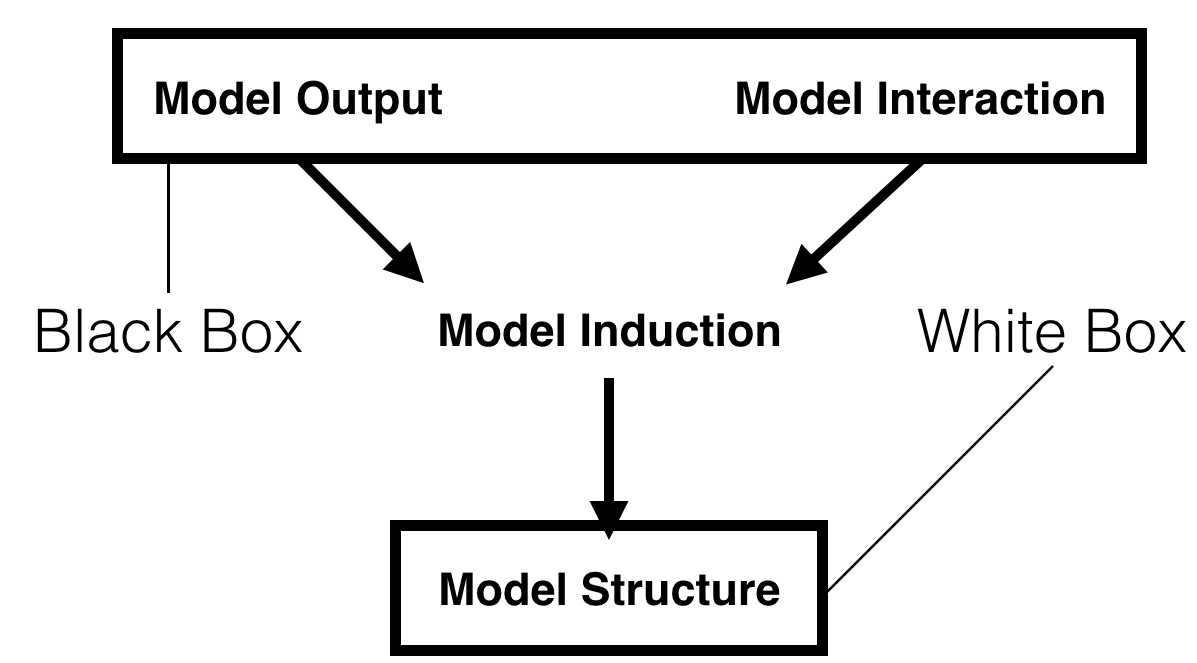
\includegraphics[height=11em]{figs/motivation/expl_classes}
\caption{
The relation of output-, interaction-, and structure-explanations.
With the help of model induction over a reduced or carefully selected
input, output- and interaction-explanations can utilize structure explanations
of simple machine learning models.
Output- and interaction-explanations can be created while treating the model
as black-box. This is not possible for structure explanations.
}
\label{figs:motivation_expl_classes}
\end{figure}

% The types of explanations can be broadly categorized into black box (output and interaction)
% and white box (structure) explanations as shown in \figref{figs:motivation_expl_classes}.
% Note that input explanations do not fall into either of those categories as they
% do not rely on any \emph{concrete} machine learning model due to focusing on data
% preparation and pre-processing.

% In this work we discuss exclusively input and black box explanations.
% Black box-, as opposed to white box-, explanations have the advantage that they can
% deal with any complexity of the underlying model.
% Developed techniques also do not need to be adapted to new algorithms emerging from
% machine learning research as long as the core interface (input produces prediction scores)
% remains the same.
% Furthermore, black box explanations also allow to compare the behavior of different
% algorithms which is otherwise not possible.
% Lastly, with good performing machine learning models being highly valued in certain
% domains stakeholders do not need to fully reveal their assets to analysts using
% black box explanations.

% \section{Overview}
% In the following we show how the previously mentioned different kinds of explanations
% can be utilized using tools we developed.

% At first we focus on tools that help with the data preparation step.
% SeekAView (see \chapref{sec:SeekAView}) helps detect unusual patterns in the data and
% provides a way to find associations between features using guided subspace analysis.
% With Patient-viz (see \chapref{sec:Patient-viz}) we show a tool to verify the integrity
% of patient records that are used to construct features for diagnosis prediction.
% The tool helped a group of machine learning modelers and practitioners refine their definitions for disease labels.
% COQUITO (see \chapref{sec:COQUITO}) is designed to ease cohort definition and construction in the medical context.

% \begin{figure}[b!]
\centering
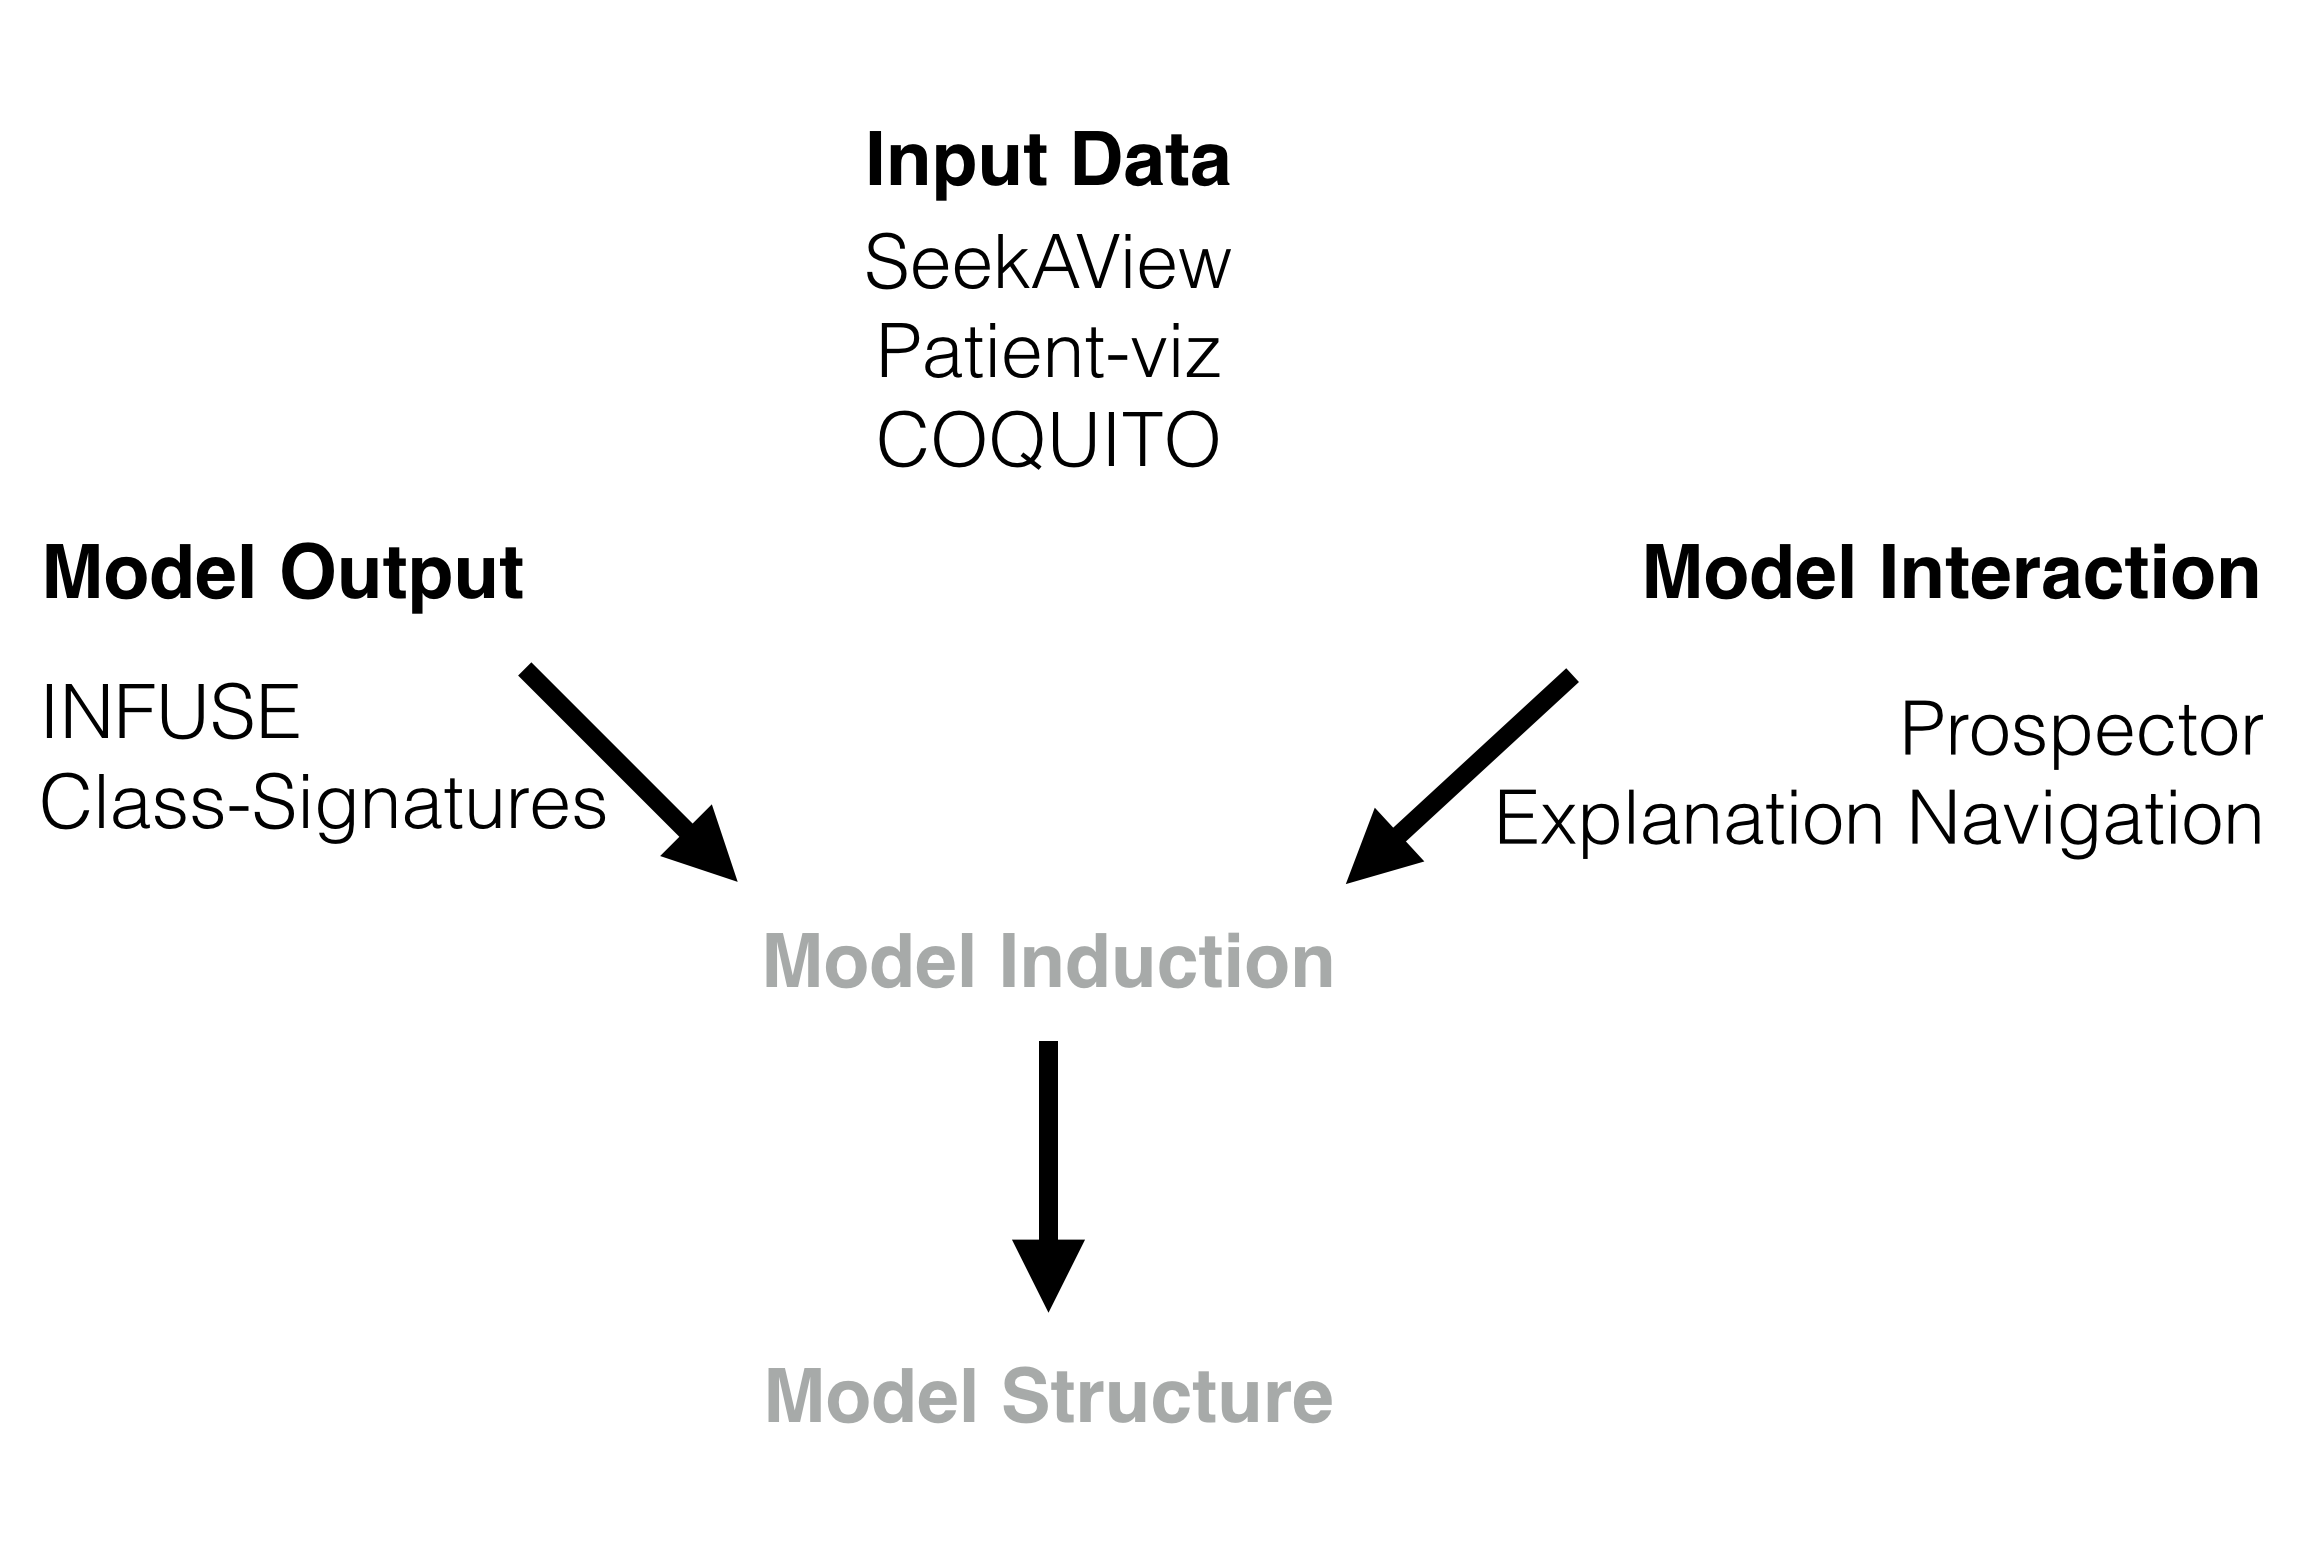
\includegraphics[height=14em]{figs/motivation/content}
\caption{
How the projects of my dissertation fit into the categorization of explanations
as shown in \figref{figs:motivation_expl_classes}.
As input data is focused on data pre-processing it doesn't appear in the
original figure. Furthermore, no works focusing on structure explanations are
presented as they require knowledge about the internal state of the model.
However, with \textbf{Class Signatures} model induction based on the original
model's outputs and subsequent structure explanations of the induced model are
part of the work-flow.
}
\label{figs:motivation_content}
\end{figure}

% Secondly, we focus on tools that use model interaction to explain model behavior.
% Those techniques search the output space of a model by manipulating the input space and differ mostly
% by their mechanism of probing the machine learning model.
% Prospector (see \chapref{sec:Prospector}) uses partial dependence to calculate the local
% influence of features.
% We are currently working on a tool that uses a different probing mechanism aimed at
% textual data which is described in \chapref{sec:Outlook}.

% Thirdly, we focus on tools using only the output of machine learning models to
% provide explanations.
% This category is especially useful if the model that produced the output cannot
% be shared or is otherwise not be available.
% The scope of model outputs can reach from feature rankings as shown with INFUSE (see \chapref{sec:INFUSE})
% to analyzing predictions scores (see \chapref{sec:Class-Signatures}).
% The latter is partially published ongoing work which we will revisit in \chapref{sec:Outlook}.

% In \chapref{sec:Outlook} we will describe current projects that fit in the categories described above.
% We further explore in which directions those projects develop and provide a time-line of their completion
% alongside a draft of final thesis' structure in \chapref{chap:outline}.
